\documentclass[10pt,landscape]{article}

\usepackage{listings}
\usepackage[italian]{babel}
\usepackage[utf8]{inputenc}
\usepackage{multicol}
\usepackage[landscape]{geometry}
\usepackage{enumitem}
\usepackage[printwatermark]{xwatermark}
\usepackage[compact]{titlesec}
\usepackage[flushleft]{threeparttable}
\usepackage{textcomp}
\usepackage{todonotes}
\usepackage{lastpage}
\usepackage{graphicx}

\geometry{top=.5in,left=.5in,right=.5in,bottom=.5in,headsep=0in}

% Turn off header and footer
\pagestyle{empty}

\definecolor{dkgreen}{rgb}{0,0.6,0}
\definecolor{gray}{rgb}{0.5,0.5,0.5}
\definecolor{mauve}{rgb}{0.58,0,0.82}

\geometry{top=.5in,left=.5in,right=.5in,bottom=.5in,headsep=0in}

% Turn off header and footer
\pagestyle{empty}

% Reduce size of \section e \subsection
\titleformat{\section}{\normalfont\large\bfseries}{\thesection}{1em}{}
\titleformat{\subsection}{\normalfont\normalsize\bfseries}{\thesubsection}{1em}{}
\titlespacing{\section}{0pt}{0ex}{-0.5ex}
\titlespacing{\subsection}{0pt}{0ex}{-0.5ex}


% Don't print section numbers
\setcounter{secnumdepth}{0}


\setlength{\parindent}{0pt}
\setlength{\parskip}{0pt plus 0.5ex}

\setlist[itemize]{noitemsep, nolistsep}


\newcommand{\rarr}{\rightarrow}

\newcommand{\cmark}{\ding{51}}%
\newcommand{\xmark}{\ding{55}}%

\pagenumbering{arabic}
\pagestyle{fancy}
\fancyhead[R]{Page \thepage{} of \pageref{LastPage}}
\fancyhead[L]{}
\fancyfoot[C]{}
\renewcommand{\headrulewidth}{0pt}



\lstset{frame=tb,
  language=Haskell,
  aboveskip=3mm,
  belowskip=3mm,
  showstringspaces=false,
  columns=flexible,
  basicstyle={\small\ttfamily},
  numbers=none,
  numberstyle=\tiny\color{gray},
  keywordstyle=\color{blue},
  commentstyle=\color{dkgreen},
  stringstyle=\color{mauve},
  breaklines=true,
  breakatwhitespace=true,
  tabsize=3
}
% \newwatermark[allpages,color=black!10,angle=45,scale=6,xpos=-20,ypos=15]{DRAFT}

\begin{document}

\raggedright
\footnotesize
\begin{multicols}{3}
% multicol parameters
% These lengths are set only within the two main columns
%\setlength{\columnseprule}{0.25pt}
\setlength{\premulticols}{1pt}
\setlength{\postmulticols}{1pt}
\setlength{\multicolsep}{1pt}
\setlength{\columnsep}{2pt}

{\Large{\textbf{Principle of Programming Languages}}}

\section{Haskell}
\section{Exams}
\subsection{2020-02-07}
Consider a data type PriceList that represents a list of items, where each item is associated with a price,
of type Float:
data PriceList a = PriceList [(a, Float)]
\begin{itemize}
	\item Make PriceList an instance of Functor and Foldable.
	\item Make PriceList an instance of Applicative, with the constraint that each application of a function in the left hand side of a <*> must increment a right hand side value’s price by the price associated with the function.
\end{itemize}
Solution:
\begin{lstlisting}
	pmap :: (a -> b) -> Float -> PriceList a -> PriceList b
	pmap f v (PriceList prices) = PriceList $ fmap (\x -> let (a, p) = x
					in (f a, p+v)) prices
	
	instance Functor PriceList where
		fmap f prices = pmap f 0.0 prices
	
	instance Foldable PriceList where
		foldr f i (PriceList prices) = foldr (\x y -> let (a, p) = x
						in f a y) i prices
	
	(PriceList x) +.+ (PriceList y) = PriceList $ x ++ y
	
	plconcat x = foldr (+.+) (PriceList []) x
	
	instance Applicative PriceList where
		pure x = PriceList [(x, 0.0)]
		(PriceList fs) <*> xs = plconcat (fmap (\ff -> let (f, v) = ff
						in pmap f v xs) fs)
\end{lstlisting}





\subsection{2020-01-15}
The following data structure represents a cash register. As it should be clear from the two accessor
functions, the first component represents the current item, while the second component is used to store
the price (not necessarily of the item: it could be used for the total). \\
\texttt{data CashRegister a = CashRegister { getReceipt :: (a, Float) } deriving (Show, Eq)} \\
\texttt{getCurrentItem = fst . getReceipt} \\
\texttt{getPrice = snd . getReceipt} \\
\begin{itemize}
    \item Make CashRegister an instance of Functor and Applicative
    \item Make CashRegister an instance of Monad.
\end{itemize}
Solution:
\begin{lstlisting}
    instance Functor CashRegister where
        fmap f cr = CashRegister (f $ getCurrentItem cr, getPrice cr)
    
    instance Applicative CashRegister where
        pure x = CashRegister (x, 0.0)
        CashRegister (f, pf) <*> CashRegister (x, px) = CashRegister (f x, pf + px)
    
    instance Monad CashRegister where
        CashRegister (oldItem, price) >>= f =
            let newReceipt = f oldItem
            in CashRegister (getCurrentItem newReceipt, price + (getPrice newReceipt))
\end{lstlisting}






\subsection{2019-09-03}
Consider the data structure Tril, which is a generic container consisting of three lists
\begin{itemize}
    \item 1) Give a data definition for Tril.
    \item 2) Define list2tril, a function which takes a list and 2 values x and y, say x < y, and builds a Tril, where the last component is the ending sublist of length x, and the middle component is the middle sublist of length y-x. Also, list2tril L x y = list2tril L y x. \\ E.g. list2tril [1,2,3,4,5,6] 1 3 should be a Tril with first component [1,2,3], second component [4,5], and third component [6].
    \item 3) Make Tril an instance of Functor and Foldable.
    \item 4) Make Tril an instance of Applicative, knowing that the concatenation of 2 Trils has first component which is the concatenation of the first two components of the first Tril, while the second component is the concatenation of the ending component of the first Tril and the beginning one of the second Tril (the third component should be clear at this point).
\end{itemize}
\begin{lstlisting}
    data Tril a = Tril [a] [a] [a] deriving (Show, Eq)

    instance Functor Tril where
        fmap f (Tril x y z) = Tril (fmap f x)(fmap f y)(fmap f z)

    instance Foldable Tril where
        foldr f i (Tril x y z) = foldr f (foldr f (foldr f i z) y) x
    
    (Tril x y z) +++ (Tril a b c) = Tril (x ++ y) (z ++ a) (b ++ c)

    trilconcat t = foldr (+++) (Tril [][][]) t
    trilcmap f t = trilconcat $ fmap f t

    instance Applicative Tril where
        pure x = Tril [x][][]
        x <*> y = trilcmap (\f -> fmap f y) x

    list2tril lst n1 n2 =   let (_,_,[x,y,z]) = foldr helper (n1, n2, [[]]) lst
                            in Tril x y z
        where
            helper el (0, m, next) = (-1, m-1, [el]:next)
            helper el (n, 0, next) = (n-1, -1, [el]:next)
            helper el (n, m, (x:xs)) = (n-1, m-1, (el:x):xs)
\end{lstlisting}




\subsection{2019-07-24}
Consider a non-deterministic finite state automaton (NFSA) and assume that its states are values of a type
State defined in some way. An NFSA is encoded in Haskell through three functions: \\
i) transition :: Char → State → [State], i.e. the transition function. \\
ii) end :: State → Bool, i.e. a functions stating if a state is an accepting state (True) or not. \\
ii) start :: [State], which contains the list of starting states. \\
\begin{itemize}
    \item 1) Define a data type suitable to encode the configuration of an NSFA.
    \item 2) Define the necessary functions (providing also all their types) that, given an automaton A (through transition, end, and start) and a string s, can be used to check if A accepts s or not.
\end{itemize}
\begin{lstlisting}
    data Config = Config String [State] deriving (Show, Eq)

    steps :: (Char -> State -> [State]) -> Config -> Bool
    steps trans (Config "" confs) = not . null $ filter end confs
    steps trans (Config (a:as) confs) = steps trans $ Config as (concatMap (trans a) confs)
\end{lstlisting}

\subsection{2019-06-28}
\begin{itemize}
    \item 1) Define a Tritree data structure, i.e. a tree where each node has at most 3 children, and every node contains a value.
    \item 2) Make Tritree an instance of Foldable and Functor.
    \item 3) Define a Tritree concatenation t1 +++ t2, where t2 is appended at the bottom-rightmost position of t1.
    \item 4) Make Tritree an instance of Applicative.
\end{itemize}
\begin{lstlisting}
    data Tritree a = Nil | Tritree a (Tritree a)(Tritree a)(Tritree a) deriving (Eq, Show)

    instance Functor Tritree where
        fmap f Nil = Nil
        fmap f (Tritree x t1 t2 t3) = Tritree (f x)(fmap f t1)(fmap f t2)(fmap f t3)

    instance Foldable Tritree where
        foldr f i Nil = i
        foldr f i (Tritree x t1 t2 t3) = f x $ foldr f (foldr f (foldr f i t3) t2) t1

    x +++ Nil = x
    Nil +++ x = x
    (Tritree x t1 t2 Nil) +++ t = (Tritree x t1 t2 t)
    (Tritree x t1 t2 t3) +++ t = (Tritree x t1 t2 (t3 +++ t))

    ttconcat t = foldr (+++) Nil t
    ttconcmap f t = ttconcat $ fmap f t

    instance Applicative Tritree where
        pure x = (Tritree x Nil Nil Nil)
        x <*> y = ttconcmap (\f -> fmap f y) x
\end{lstlisting}

\subsection{2019-02-08}
We want to define a data structure, called BFlist (Back/Forward list), to define lists that can either be “forward” (like usual list, from left to right), or “backward”, i.e. going from right to left. \\
We want to textually represent such lists with a plus or a minus before, to state their direction: e.g. +[1,2,3] is a forward list, -[1,2,3] is a backward list. \\
Concatenation (let us call it $<++>$) for BFlist has this behavior: if both lists have the same direction, the returned list is the usual concatenation. Otherwise, forward and backward elements of the two lists delete each other, without considering their stored values. \\
For instance: +[a,b,c] $<++>$ -[d,e] is +[c], and -[a,b,c] $<++>$ +[d,e] is -[c].
\begin{itemize}
    \item 1) Define a datatype for BFlist.
    \item 2) Make BFList an instance of Eq and Show, having the representation presented above.
    \item 3) Define $<++>$, i.e. concatenation for BFList.
    \item 4) Make BFList an instance of Functor.
    \item 5) Make BFList an instance of Foldable.
    \item 6) Make BFList an instance of Applicative.
\end{itemize}
\begin{lstlisting}
    data Dir = Fwd | Bwd deriving Eq
    data BFlist a = BFlist Dir [a] deriving Eq

    instance Show Dir where
        show Fwd = "+"
        show Bwd = "-"

    instance (Show a) => Show (BFlist a) where
        show (BFlist x y) = show x ++ show y
    instance Functor BFlist where
        fmap f (BFlist d x) = BFlist d (fmap f x)

    instance Foldable BFlist where
        foldr f i (BFlist d x) = foldr f i x
    
    (BFlist _ []) <++> x = x
    x <++> (BFlist _ []) = x
    (BFlist d1 x) <++> (BFlist d2 y) | d1 == d2 = BFlist d1 (x ++ y)
    (BFlist d1 (x:xs)) <++> (BFlist d2 (y:ys)) = (BFlist d1 xs) <++> (BFlist d2 ys)
    
    bflconcat (BFlist d v) = foldr (<++>) (BFlist d []) (BFlist d v)
    bflconcatmap f x = bflconcat $ fmap f x
    
    instance Applicative BFlist where
        pure x = BFlist Fwd [x]
        x <*> y = bflconcatmap (\f -> fmap f y) x
\end{lstlisting}

 
\subsection{2019-01-16}
We want to define a data structure, called Listree, to define structures working both as lists and as binary
trees, like in the next figure.
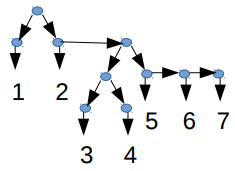
\includegraphics{haskell/2019-02-08.png}
\begin{itemize}
    \item 1) Define a datatype for Listree.
    \item 2) Write the example of the figure with the defined data structure.
    \item 3) Make Listree an instance of Functor.
    \item 4) Make Listree an instance of Foldable.
    \item 5) Make Listree an instance of Applicative.
\end{itemize}
\begin{lstlisting}
    data Listree a = Nil | Cons a (Listree a) | Branch (Listree a)(Listree a) deriving (Eq, Show)

    exfig = Branch (Cons 1 Nil) (Cons 2 (Branch (Branch (Cons 3 Nil) (Cons 4 Nil)) (Cons 5 (Cons 6 (Cons 7 Nil)))))

    instance Functor Listree where
        fmap f Nil = Nil
        fmap f (Cons x y) = Cons (f x) (fmap f y)
        fmap f (Branch x y) = Branch (fmap f x) (fmap f y)

    instance Foldable Listree where
        foldr f i Nil = i
        foldr f i (Cons x y) = f x (foldr f i y)
        foldr f i (Branch x y) = foldr f (foldr f i x) y

    x <++> Nil = x
    Nil <++> x = x
    (Cons x y) <++> z = (Cons x (y <++> z))
    (Branch x y) <++> z = (Branch x (y <++> z))

    ltconcat t = foldr (<++>) Nil t
    ltconcmap f t = ltconcat $ fmap f t

    instance Applicative Listree where
        pure x = (Cons x Nil)
        x <*> y = ltconcmap (\f -> fmap f y) x
\end{lstlisting}


\subsection{2018-07-06}
Consider this datatype: \texttt{data Blob a = Blob a (a -> a)} \\
Note: in this exercise, do not consider the practical meaning of Blob; the only constraint is to use all the available data, and the
types must be right! \\
E.g. \\
\texttt{instance Show a => Show (Blob a) where} \\
 \texttt{show (Blob x f) = "Blob " ++ (show (f x))}
\begin{itemize}
    \item 1) Can Blob automatically derive Eq? Explain how, why, and, if the answer is negative, make it an instance of Eq.
    \item 2) Make Blob an instance of the following classes: Functor, Foldable, and Applicative.
\end{itemize}
Solution:
\begin{lstlisting}
    instance Eq a => Eq (Blob a) where
        (Blob x f) == (Blob y g) = (f x) == (g y)
    instance Functor Blob where
        fmap f (Blob x g) = Blob (f (g x)) id

    instance Foldable Blob where
        foldr f z (Blob x g) = f (g x) z
    instance Applicative Blob where
        pure x = Blob x id
        (Blob fx fg) <*> (Blob x g) = Blob (((fg fx) . g) x) id
\end{lstlisting}
\section{Exercise session}
\subsection{2019-10-29}
\begin{lstlisting}[language=Haskell]
module ES20191029 where

-- Factorial in Haskell
fact :: Int -> Int
fact 0 = 1
fact n = n * fact (n-1)

facti :: Integer -> Integer
facti 0 = 1
facti n = n * facti (n-1)
-- Int is a fixed-precision integer type with at least the range [-2^29 .. 2^29-1].
-- Integer are arbitrary-precision integers.

-- Fibonacci in Haskell
fib :: Integer -> Integer
fib 0 = 0
fib 1 = 1
fib n = fib (n-1) + fib (n-2)

-- We can use guards, too
fibg :: Integer -> Integer
fibg n | n == 0 = 0
       | n == 1 = 1
       | otherwise = fibg (n-1) + fibg (n-2)

-- A few functions with lists
myLength :: [a] -> Int
myLength [] = 0
myLength (x : xs) = 1 + myLength xs

empty :: [a] -> Bool
empty [] = True
empty (_:_) = False

myReverse :: [a] -> [a]
myReverse [] = []
myReverse (x:xs) = myReverse xs ++ [x]

range :: Integer -> Integer -> [Integer]
range a b = if a > b
  then error "Min > Max"
  else if a < b
       then a : (range (a+1) b)
       else [a]

range2 :: Integer -> Integer -> [Integer]
range2 a b | a > b =  error "Min > Max"
           | a < b = a : (range (a+1) b)
           | otherwise = [a]

-- List comprehensions
rightTriang n = [(a, b, c) | a <- [1..n], b <- [1..a], c <- [1..b], a^2 == b^2 + c^2]

allRightTriang = [(a, b, c) | a <- [1..], b <- [1..a], c <- [1..b], a^2 == b^2 + c^2]

-- We can make an infinite list this way, too.
numsfrom :: Integer -> [Integer]
numsfrom n = n : (numsfrom $ n+1)

-- Alternatively:
numsfrom2 n = [n, n+1 ..]

-- fib 100 is very slow...
fibinf = 0 : 1 : [x + y | (x,y) <- zip fibinf $ tail fibinf]
-- try take 10 $ zip fibinf $ tail fibinf
-- try fib 100 and take 100 fibinf

fibb n = fibb' n (0,1)
  where fibb' n (f1, f2) | n == 0 = f1
                         | otherwise = (fibb' $! (n-1)) $! (f2, f1+f2)

-- ($!) f $! x = seq x (f x)

-- Higher order functions
myMap :: (a -> b) -> [a] -> [b]
myMap _ [] = []
myMap f (x:xs) = f x : (myMap f xs)

myTakeWhile :: (a -> Bool) -> [a] -> [a]
myTakeWhile _ [] = []
myTakeWhile p (x:xs) = if p x
  then x : myTakeWhile p xs
  else []


data TrafficLight = Red | Green | Yellow deriving (Show, Eq)

-- instance Show TrafficLight where
--   show Red = "Red light"
--   show Yellow = "Yellow light"
--   show Green = "Green light"

-- instance Eq TrafficLight where
--   Red == Red = True
--   Yellow == Yellow = True
--   Green == Green = True
--   _ == _ = False

-- Sum type
data Point = Point Float Float deriving (Eq, Show)

pointx (Point x _) = x
pointy (Point _ y) = y

distance :: Point -> Point -> Float
distance (Point x1 x2) (Point y1 y2) =
  let d1 = x1-y1
      d2 = x2-y2
  in sqrt $ (d1*d1) + (d2*d2)

type TPoint = (Float, Float)

tdistance :: TPoint -> TPoint -> Float
tdistance (x1, x2) (y1, y2) =
  let d1 = x1-y1
      d2 = x2-y2
  in sqrt $ (d1*d1) + (d2*d2)

data APoint = APoint {apx, apy :: Float} deriving (Eq, Show)
\end{lstlisting}
\subsection{2019-11-12}
\begin{lstlisting}[language=Haskell]
module ES5 where

-- A few more higher order functions

-- map
-- map (+1) [1..10]

-- filter
-- filter even [1..100]
myFilter :: (a -> Bool) -> [a] -> [a]
myFilter _ [] = []
myFilter p (x:xs) | p x = x : myFilter p xs
                  | otherwise = myFilter p xs

-- zip
-- zip [1..10] ['a'..'j']
myZip :: [a] -> [b] -> [(a, b)]
myZip l [] = []
myZip [] l = []
myZip (x:xs) (y:ys) = (x, y) : myZip xs ys

-- myZip [1,2,3] ['a','b','c']

-- zipWith
-- zipWith (*) [1..10] [1..10]

myZipWith _ _ [] = []
myZipWith _ [] _ = []
myZipWith f (x:xs) (y:ys) = f x y : myZipWith f xs ys

myFoldL :: (b -> a -> b) -> b -> [a] -> b
myFoldL _ acc [] = acc
myFoldL f acc (x:xs) = myFoldL f (f acc x) xs
-- myFoldL (+) 0 [1,2,3]

myFoldR :: (a -> b -> b) -> b -> [a] -> b
myFoldR _ acc [] = acc
myFoldR f acc (x:xs) = f x $ myFoldR f acc xs

-- we can use folds to redefine many higher order functions
sumf :: Num n => [n] -> n
sumf = foldl (+) 0

elem' e = foldl (\acc x -> x == e || acc) False
-- what's the type of elem'?
-- elem' 2 [1..10]
-- elem' 100 [1..10]

filter' :: (a -> Bool) -> [a] -> [a]
filter' p = foldr
  (\x acc -> if p x then x : acc else acc)
  []
-- filterf odd [1..10]

map' f = foldr (\x acc -> (f x): acc) []

map'' f = foldl (\acc x -> acc ++ [f x]) []
-- map'' (+3) [1..10]

-- Try foldr (:) [] [1..10]
-- this is the identity

lapp :: [a] -> [a] -> [a]
lapp l1 l2 = foldr (:) l2 l1
-- lapp [1..10] [20..100]
-- [1..10] ++ [20..100]

takeWhile' p = foldr (\x acc -> if p x then x:acc else []) []
-- it works with infinite lists too
-- takeWhile' (<10) [1..]

-- Binary Tree
data BTree a = BEmpty | BNode a (BTree a) (BTree a)

instance Eq a => Eq (BTree a) where
  BEmpty == BEmpty = True
  BNode x1 l1 r1 == BNode x2 l2 r2 =
    x1 == x2 && l1 == l2 && r1 == r2
  _ == _ = False

instance Show a => Show (BTree a) where
  show BEmpty = "Empty"
  show (BNode x BEmpty BEmpty) = "BNode " ++ show x
  show (BNode x l r) = "BNode " ++ show x ++ " (" ++ show l ++ ") (" ++ show r ++ ")"

bleaf x = BNode x BEmpty BEmpty

isbleaf (BNode _ BEmpty BEmpty) = True
isbleaf _ = False

btmap :: (a -> b) -> BTree a -> BTree b
btmap _ BEmpty = BEmpty
btmap f (BNode x l r) =
  BNode (f x) (btmap f l) (btmap f r)
-- btmap (*2) (BNode 1 BEmpty BEmpty)
-- btmap (*2) (BNode 1 (bleaf 2) (bleaf 3))

instance Functor BTree where
  fmap = btmap

-- Functor laws:
-- fmap id = id
-- fmap (f . g) = fmap f . fmap g
-- Indeed:
-- fmap id (BNode 1 BEmpty BEmpty)
-- fmap id (BNode 1 (bleaf 2) (bleaf 3))
-- and
-- fmap (*2) $ fmap (+1) (BNode 1 (bleaf 2) (bleaf 3))
-- fmap ((*2) . (+1)) (BNode 1 (bleaf 2) (bleaf 3))

btfoldr :: (a -> b -> b) -> b -> BTree a -> b
btfoldr _ acc BEmpty = acc
btfoldr f acc (BNode x l r) =
  f x (btfoldr f (btfoldr f acc r) l)
-- btfoldr (+) 0 (BNode 6 (bleaf 1) (bleaf 2))

instance Foldable BTree where
  foldr = btfoldr

-- Count nodes:
-- foldr (\_ acc -> acc + 1) 0 (BNode 6 (bleaf 1) (bleaf 2))

-- Depth-First Visit:
-- foldr (:) [] (BNode 6 (bleaf 1) (bleaf 2))

-- DFS:
btelem x = foldr (\y acc -> x == y || acc) False

-- infinite trees
inftree n = BNode n (inftree (n+1)) (inftree (n+1))

bttake _ BEmpty = BEmpty
bttake h (BNode x l r)
  | h <= 0 = BEmpty
  | otherwise = BNode x (bttake (h-1) l) (bttake (h-1) r)

btZipWith _ _ BEmpty = BEmpty
btZipWith _ BEmpty _ = BEmpty
btZipWith f (BNode x1 l1 r1) (BNode x2 l2 r2) =
  BNode (f x1 x2) (btZipWith f l1 l2) (btZipWith f r1 r2)
\end{lstlisting}
\subsection{2019-11-19}
\begin{lstlisting}[language=Haskell]
module ES6 where

import qualified Data.Map as M

data BTree a = BEmpty | BNode a (BTree a) (BTree a) deriving Eq

instance (Show a) => Show (BTree a) where
  show BEmpty = "Bempty"
  show (BNode x BEmpty BEmpty) = "BNode " ++ show x
  show (BNode x l r) = "BNode " ++ show x ++ " (" ++ show l ++ ") (" ++ show r ++ ")"

bleaf x = BNode x BEmpty BEmpty

isbleaf (BNode _ BEmpty BEmpty) = True
isbleaf _ = False

btmap :: (a -> b) -> BTree a -> BTree b
btmap _ BEmpty = BEmpty
btmap f (BNode x l r) = BNode (f x) (btmap f l) (btmap f r)

instance Functor BTree where
  fmap = btmap

-- fmap can be seen as "apply f to all elements of a container/context"
-- fmap (+1) $ Just 42
-- fmap (+1) Nothing
-- fmap (+1) [1..10]
-- fmap (+1) (BNode 1 (bleaf 2) (bleaf 3))

-- but also as a way to lift a unary function, so that it works between functors
-- :t fmap
-- :t fmap (+1)
incAll :: (Functor f, Num b) => f b -> f b
incAll = fmap (+1)
-- inc $ Just 1
-- inc [1..9]
-- inc (BNode 1 (bleaf 2) (bleaf 3))

-- class (Functor f) => Applicative f where
--   pure :: a -> f a
--   (<*>) :: f (a -> b) -> f a -> f b

-- pure encloses something into an applicative in a default way
-- pure 42 :: Maybe Integer
-- pure 42 :: [Integer]

-- <*> takes an applicative containing a function, and applies it to the content of another applicative
-- pure (*2) <*> Just 42
-- pure (*2) <*> [1..10]
-- now we can apply general functions to containers/contexts
-- pure (*) <*> Just 6 <*> Just 7
-- pure (\x y z -> x*y*z) <*> Just 2 <*> Just 3 <*> Just 4
-- pure (\x y z -> x*y*z) <*> Just 2 <*> Nothing <*> Just 4

-- (fmap (\x y z -> x*y*z) (Just 2)) <*> Just 3 <*> Just 4
-- (fmap (\x y z -> x*y*z) (Just 2)) <*> Nothing <*> Just 4

-- To make this simpler, we have <$>:
-- (<$>) :: (Functor f) => (a -> b) -> f a -> f b
-- f <$> x = fmap f x

-- (*) <$> Just 6 <*> Just 7
-- (\x y z -> x*y*z) <$> Just 2 <*> Just 3 <*> Just 4
-- (\x y z -> x*y*z) <$> Just 2 <*> Nothing <*> Just 4

-- With lists:
-- (+2) <$> [1..3]
-- (+) <$> [1..3] <*> [2]
-- (+) <$> [1..3] <*> [1..10]
-- [(+1), (+2), (+3)] <*> [1..10]

-- this is due to the peculiar implementation of Applicative for lists
concat' [] = []
concat' (x:xs) = x ++ concat' xs

concatMap' f l = concat' $ map f l

-- instance Applicative [] where
--   pure x = [x]
--   fs <*> xs = concatMap' (\f -> map f xs) fs

-- But this is not the only way of implementing Applicative for lists
data ZipList a = ZEmpty | ZL a (ZipList a)

instance (Eq a) => Eq (ZipList a) where
  ZEmpty == ZEmpty = True
  ZL x xs == ZL y ys = x == y && xs == ys
  _ == _ = False

showZipList ZEmpty = "[]"
showZipList (ZL x ZEmpty) = "[" ++ show x ++ "]"
showZipList (ZL x xs) = "[" ++ show x ++ "," ++ (drop 1 $ showZipList xs)

instance (Show a) => Show (ZipList a) where
  show l = "ZipList " ++ showZipList l

instance Functor ZipList where
  fmap _ ZEmpty = ZEmpty
  fmap f (ZL x xs) = ZL (f x) $ fmap f xs

toZipList :: [a] -> ZipList a
toZipList [] = ZEmpty
toZipList (x:xs) = ZL x (toZipList xs)

instance Applicative ZipList where
  pure x = ZL x $ pure x
  ZEmpty <*> _ = ZEmpty
  _ <*> ZEmpty = ZEmpty
  ZL f fs <*> ZL y ys = ZL (f y) (fs <*> ys)

-- (toZipList [(+1), (+2), (*3)]) <*> (toZipList [1,2,3])
-- pure (*1) <*> toZipList [1..10] -- meh

-- Let us make binary trees Applicative
btcat BEmpty t2 = t2
btcat t1 BEmpty = t1
btcat t1@(BNode x l r) t2 = BNode x l new_r
  where new_r = if isbleaf t1
                then t2
                else btcat r t2
-- btcat (BNode 1 (bleaf 2) (bleaf 3)) (BNode 4 (bleaf 5) (bleaf 6))

btfoldr _ acc BEmpty = acc
btfoldr f acc (BNode x l r) =
  f x (btfoldr f (btfoldr f acc r) l)

btconcat t = btfoldr btcat BEmpty t

btcatmap f t = btconcat $ fmap f t
-- btcatmap (\x -> BNode x (bleaf x) (bleaf x)) (BNode 1 (bleaf 2) (bleaf 3))

-- instance Applicative BTree where
--   pure = bleaf
--   fs <*> xs = btcatmap (\f -> fmap f xs) fs

-- we can also do it with the Zip semantics
instance Applicative BTree where
  pure x = BNode x (pure x) (pure x)
  BEmpty <*> _ = BEmpty
  _ <*> BEmpty = BEmpty
  BNode f lf rf <*> BNode x lx rx = BNode (f x) (lf <*> lx) (rf <*> rx)


-- An exercise on Data.Map
-- map(personNames, PhoneNumbers)
-- map(PhoneNumber, MobileCarriers)
-- map(MobileCarriers, BillingAddresses)

type PersonName = String
type PhoneNumber = String
type BillingAddress = String
data MobileCarrier = TIM | Vodafone | Wind | Iliad deriving (Eq, Show, Ord)


findCarrierBillingAddress ::
  PersonName
  -> M.Map PersonName PhoneNumber
  -> M.Map PhoneNumber MobileCarrier
  -> M.Map MobileCarrier BillingAddress
  -> Maybe BillingAddress
findCarrierBillingAddress person phoneMap carrierMap addressMap =
  case M.lookup person phoneMap of
    Nothing -> Nothing
    Just number ->
      case M.lookup number carrierMap of
        Nothing -> Nothing
        Just carrier -> M.lookup carrier addressMap

findCarrierBillingAddress' person phoneMap carrierMap addressMap =
  do
    number <- M.lookup person phoneMap
    carrier <- M.lookup number carrierMap
    M.lookup carrier addressMap
\end{lstlisting}
\subsection{2019-11-26}
\begin{lstlisting}[language=Haskell]
module ES7 where

-- We saw:
-- Functors, to lift a function so that it works on a container/context
-- fmap (+2) (Just 5)
-- :t fmap (+2)
-- Applicative, to do the same with functions with multiple arguments
-- (+) <$> Just 5 <*> Just 2

-- What if we have a function that *returns* a value wrapped in a container/context?
apply42 f x = let s = f x
              in if s > 42 then Just s else Nothing

-- we want to apply a sequence of functions to an initial value,
-- but none of them can return a value lower than 42.
sequence42 x = case apply42 (+12) x of
  Nothing -> Nothing
  Just x1 -> case apply42 (\x -> x-6) x1 of
    Nothing -> Nothing
    Just x2 -> apply42 (*2) x2

-- Try sequence42 42
-- sequence42 30

-- We must combine the information in the context containing the input value
-- with the context generated by the function in the output value.

-- class Monad m where
--   return :: a -> m a
--   (>>=) :: m a -> (a -> m b) -> m b
--   (>>) :: m a -> m b -> m b
--   x >> y = x >>= \_ -> y
--   fail :: String -> m a
--   fail msg = error msg

-- instance Monad Maybe where
--   return x = Just x
--   Nothing >>= f = Nothing
--   Just x >>= f  = f x
--   fail _ = Nothing

sequence42' x = return x
  >>= apply42 (+12)
  >>= apply42 (\x -> x-6)
  >>= apply42 (*2)

-- do notation:
sequence42do x = do
  x1 <- apply42 (+12) x
  x2 <- apply42 (\x -> x-6) x1
  x3 <- apply42 (*2) x2
  return x3

-- this gets translated to
sequence42do' x = apply42 (+12) x >>=
  (\x1 -> apply42 (\x -> x-6) x1 >>=
    (\x2 -> apply42 (*2) x2 >>=
      (\x3 -> return x3)))

sequenceDiscard x = do
  apply42 (+1) x
  x1 <- apply42 (*2) x
  return x1

-- this is the same as
sequenceDiscard' x = apply42 (+1) x >> apply42 (*2) x
  >>= (\x1 -> return x1)

sequenceDiscard'' x = apply42 (+1) x >>=
  (\_ -> apply42 (*2) x >>= (\x1 -> return x1))

-- Let's make a Monad ourselves!
-- The Log Monad
type Log = [String]
newtype Logger a = Logger { unwrap :: (a, Log) }

getContent l = x where (x, _) = unwrap l
getLog l = log where (_, log) = unwrap l

instance (Eq a) => Eq (Logger a) where
  Logger (x, _) == Logger (y, _) = x == y

instance (Show a) => Show (Logger a) where
  show l = show (getContent l)
    ++ "\n\nLog:"
    ++ foldr (\line acc -> "\n\t" ++ line ++ acc)
             ""
             (getLog l)

instance Functor Logger where
  fmap f l = let (x, log) = unwrap l
             in Logger (f x, log)

-- Functor laws:
-- fmap id = id
-- fmap (f . g) = fmap f . fmap g
-- what if we modified the log?

instance Applicative Logger where
  pure x = Logger (x, [])
  Logger (f, lf) <*> Logger (x, lx) =
    Logger (f x, lf ++ lx)

-- (+) <$> Logger (2, ["first operand: 2"]) <*> Logger (3, ["second operand: 3"])

instance Monad Logger where
  return = pure
  Logger (x, log) >>= f = let (y, newLog) = unwrap $ f x
                          in Logger (y, log ++ newLog)

logPlusOne :: (Num a) => a -> Logger a
logPlusOne x = Logger (x+1, ["Add one."])

logMultiplyTwo x = Logger (x*2, ["Multiply by two."])

doOps x = do
  x1 <- logPlusOne x
  logMultiplyTwo x1
  x3 <- logPlusOne x1
  return x3

-- Monadic Laws
-- Left identity: return a >>= f 'equivalent to' f a
-- f has the type (a -> m b) so it returns a monad
-- this means that the minimal context to return 
-- is just applying f to a

-- return 42 >>= logPlusOne
-- logPlusOne 42

-- Right identity: m >>= return 'equivalent to' m
-- When we feed monadic values to functions by using >>=, 
-- those functions take normal values and return monadic ones. 
-- return is also one such function, if you consider its type.

-- Logger (1,["barnibalbi"]) >>= return

-- Associativity:  (m >>= f) >>= g 'equivalent to' m >>= (\x -> f x >>= g)

doOps' x = logPlusOne x >>=
  (\x1 -> logMultiplyTwo x1 >>=
    (\x2 -> logPlusOne x2 >>=
      (\x3 -> return x3)))
-- doOps 3 is the same as
-- doOps' 3


-- Let us take our binary trees again
data BTree a = BEmpty | BNode a (BTree a) (BTree a) deriving Eq

instance (Show a) => Show (BTree a) where
  show BEmpty = "BEmpty"
  show (BNode x BEmpty BEmpty) = "BNode " ++ show x
  show (BNode x l r) = "BNode "++ show x ++ " (" ++ show l ++ ") (" ++ show r ++ ")"

bleaf x = BNode x BEmpty BEmpty

putLog :: String -> Logger ()
putLog msg = Logger ((), [msg])

bleafM x = do
  putLog $ "Create leaf " ++ show x
  return $ bleaf x

treeReplaceM :: (Show a) => (BTree a) -> (a -> Bool) -> a
  -> Logger (BTree a)
treeReplaceM BEmpty _ _ = return BEmpty
treeReplaceM (BNode x l r) p y = do
  newL <- treeReplaceM l p y
  newR <- treeReplaceM r p y
  if p x
  then do
    putLog $ "Replaced " ++ show x ++ " with " ++ show y
    return $ BNode y newL newR
  else do
    return $ BNode x newL newR

-- This is the same as
-- treeReplaceM (BNode x l r) p y =
--   treeReplaceM l p y >>=
--   (\newL -> treeReplaceM r p y >>=
--             (\newR -> if p x
--               then do
--                 putLog $ "Replaced " ++ show x ++ " with " ++ show y
--                 return $ BNode y newL newR
--               else
--                 return $ BNode x newL newR))
\end{lstlisting}
\subsection{2019-12-03}
\begin{lstlisting}[language=Haskell]
module ES8 where

import Control.Monad.Fail

-- Exam 2017 02 27
data LolStream x = LolStream Int [x]

-- The list [x] must always be an infinite list
-- (also called a stream), while the first parameter, of type Int,
-- when positive represents the fact that the stream is periodic, while it is not periodic if
-- negative (0 is left unspecified). E.g.
-- LolStream -1 [1,2..]
-- LolStream 2 [1,2,1,2...]
period12 = [1,2] ++ period12
-- LolStream 2 period12

isperiodic (LolStream n _) = n > 0
destream ls@(LolStream n l) = if isperiodic ls
  then take n l
  else l

instance (Eq a) => Eq (LolStream a) where
  ls1 == ls2 = destream ls1 == destream ls2

instance (Show a) => Show (LolStream a) where
  show = show . destream

-- Define a function lol2lolstream which takes a finite list of finite lists
-- [h 1 , h 2 , ... h n ], and returns
-- LolStream (|h 1 | + |h 2 | + ... + |h n |) (h 1 ++ h 2 ++ ... ++ h n ++ h 1 ++ h 2 ++ ...)
lolrepeat xs = xs ++ lolrepeat xs

lol2lolstream :: [[a]] -> LolStream a
lol2lolstream ls = let lscat = foldr (++) [] ls
                   in LolStream (length lscat) (lolrepeat lscat)

instance Functor LolStream where
  fmap f (LolStream n l) = LolStream n $ map f l

instance Foldable LolStream where
  foldr f e ls = foldr f e $ destream ls

instance Applicative LolStream where
  pure x = lol2lolstream [[x]]
  ls1@(LolStream nf fs) <*> ls2@(LolStream nx xs) =
    LolStream (nf * nx) $ lolrepeat (destream ls1 <*> destream ls2)

-- lol2lolstream [[(+2),(*3)]] <*> lol2lolstream [[1..4]]

instance Monad LolStream where
  ls >>= f = lol2lolstream [destream ls >>= \x -> destream (f x)]


something = do
  x <- lol2lolstream [[1..3]]
  y <- lol2lolstream [[2..4]]
  return (x,y)

somethingButWithLists = do
  x <- [1..3]
  y <- [2..4]
  return (x,y)


-- Let us try to implement a stack in Haskell.
type Stack = [Int]

pop :: Stack -> (Stack, Int)
pop [] = error "Popping an empty stack!"
pop (x:xs) = (xs, x)

push :: Int -> Stack -> (Stack, ())
push x xs = (x:xs, ())

-- Define a function that executes the following operations on the stack:
-- pop an element
-- pop another element
-- push 100
-- pop an element
-- push 42
stackManip :: Stack -> (Stack, ())
stackManip stack = let
  (newStack1, a) = pop stack
  (newStack2, b) = pop newStack1
  (newStack3, ()) = push 100 newStack2
  (newStack4, c) = pop newStack3
  in push 42 newStack4
-- try stackManip [1..10]

data State st a = State (st -> (st, a))

instance Functor (State st) where
  fmap f (State g) = State (\s -> let (s', x) = g s
                                  in  (s', f x))

instance Applicative (State st) where
  pure x = State (\t -> (t, x))
  (State f) <*> (State g) =
    State (\state -> let (s, f') = f state
                         (s', x) = g s
                     in  (s', f' x))

instance Monad (State state) where
  State f >>= g = State (\olds ->
                           let (news, value) = f olds
                               State f' = g value
                           in f' news)

-- We need this to use the do notation with pattern matching since GHC 8.6.1.
instance MonadFail (State a) where
  fail s = error s

runStateM :: State state a -> state -> (state, a)
runStateM (State f) st = f st

getState = State (\state -> (state, state))
putState new = State (\_ -> (new, ()))

-- define pop using the State monad
popM :: State Stack Int
popM = do
  (x:xs) <- getState
  putState xs
  return x

-- define push using the State monad
pushM :: Int -> State Stack ()
pushM x = do
  xs <- getState
  putState (x:xs)
  return ()

stackManipM :: State Stack ()
stackManipM = do
  popM
  popM
  pushM 100
  popM
  pushM 42

-- runStateM stackManipM [1..10]


-- Exam 2015 09 22
-- Define the Bilist data-type, which is a container of two homogeneous lists.
-- Define an accessor for Blist, called bilist_ref, that, given an index i, 
-- returns the pair of values at position i in both lists.
-- E.g. bilist_ref (Bilist [1,2,3] [4,5,6]) 1 should return (2,5).
data Bilist a = Bilist [a] [a] deriving (Eq, Show)

bilist_ref (Bilist l1 l2) n = (l1 !! n, l2 !! n)

-- Define a function, called oddeven, that is used to build a Bilist x y from a simple list. 
-- oddeven takes all the elements at odd positions and puts them in y, 
-- while all the other elements are put in x, maintaining their order. 
-- You may assume that the given list has an even length (or 0). 
-- Write also all the types of the functions you define.
-- E.g. oddeven [1,2,3,4] must be Bilist [1,3] [2,4].
oddeven :: [a] -> Bilist a
oddeven l = oddevenh l [] []
  where oddevenh [] ev od = Bilist ev od
        oddevenh (x:xs) ev od = oddevenh xs od (ev ++ [x])

inv_oddeven :: Bilist a -> [a]
inv_oddeven (Bilist l r) =  concat $ map (\(x,y) -> [x,y]) $ zip l r


bilist_maxh :: (Num a, Ord a) => Bilist a -> Int -> a -> Int -> Int
bilist_maxh (Bilist (l:ls) (r:rs)) pos max maxpos
  | l+r > max = bilist_maxh (Bilist ls rs) (pos+1) (l+r) pos
  | otherwise = bilist_maxh (Bilist ls rs) (pos+1) max maxpos
bilist_maxh _ _ _ maxpos = maxpos

bilist_max (Bilist (l:ls) (r:rs)) =
  bilist_maxh (Bilist ls rs) 1 (l+r) 0

-- Try to make Bilist an instance of Functor, Foldable, Applicative, Monad.
\end{lstlisting}



\rule{0.3\linewidth}{0.25pt}
\end{multicols}
\end{document}